\documentclass[conference]{IEEEtran}
\IEEEoverridecommandlockouts
\usepackage{cite}
\usepackage{amsmath,amssymb,amsfonts}
\usepackage{algorithmic}
\usepackage{graphicx}
\usepackage{booktabs}
\usepackage{float}
\usepackage{subfig}
\usepackage{textcomp}
\usepackage{xcolor}
\def\BibTeX{{\rm B\kern-.05em{\sc i\kern-.025em b}\kern-.08em
    T\kern-.1667em\lower.7ex\hbox{E}\kern-.125emX}}
\begin{document}

\title{Thermal Risk Monitoring in Electric Vehicle Batteries Using External Sensors and Machine Learning Algorithms}

\author{\IEEEauthorblockN{Hítalo Bruno de Azevedo Nascimento}
\IEEEauthorblockA{\textit{Centro de informática} \\
\textit{Universidade Federal de Pernambuco}\\
Recife, Brazil \\
hban@cin.ufpe.br}
}

\maketitle

\begin{abstract}
Thermal safety remains a critical challenge for electric vehicles, as abnormal temperature evolution in lithium ion batteries may lead to severe degradation or catastrophic failure. Conventional battery thermal monitoring is primarily performed by the Battery Management System, which relies on internal sensors, fixed thresholds, and proprietary data access. These characteristics limit adaptability to real world operating conditions and restrict deployment in retrofitted or third party scenarios.

This paper presents a machine learning-based approach for battery thermal monitoring and early thermal risk awareness using exclusively external, non-intrusive temperature sensing. A low-cost sensing architecture based on an ESP32 microcontroller was developed to collect battery surface temperature, ambient temperature, and operational data during real-world riding experiments with an electric motorcycle. The collected telemetry was transmitted via a mobile gateway and processed in a backend infrastructure for time series analysis.

Battery thermal behavior was modeled as a forecasting problem, and multiple machine learning algorithms, including K Nearest Neighbors, Decision Trees, Random Forest, Gradient Boosting, and Multilayer Perceptron, were evaluated. Results demonstrate that forecasting-based models can accurately capture battery surface temperature evolution when temporal features are incorporated, despite minor data losses and measurement noise.

The findings indicate that external surface temperature measurements combined with time series forecasting can provide meaningful early thermal trend awareness without reliance on internal Battery Management System signals. This approach offers a practical, deployable, and non intrusive complementary safety layer for real world electric vehicle battery monitoring.
\end{abstract}

\begin{IEEEkeywords}
battery thermal monitoring, external temperature sensing, non-intrusive monitoring, time series forecasting, machine learning, electric motorcycles, real-world experiments
\end{IEEEkeywords}

\section{Introduction}
The thermal safety of electric vehicles (EVs) represents one of the most critical challenges currently faced by the automotive industry, as phenomena such as thermal runaway can lead to uncontrollable fires, severe material damage, and significant risks to human life (Feng et al., 2018; Li et al., 2023). Battery thermal monitoring is traditionally performed through the Battery Management System (BMS), which relies on internal sensors to supervise cell and module temperatures and to enforce operational safety limits (Pesaran et al., 2017). However, these systems commonly depend on fixed thresholds or lookup tables derived from laboratory-based testing, which constrains their adaptability to the dynamic conditions of real-world operation and to the progressive aging of battery cells (Xie et al., 2020; Hong et al., 2022).

In addition, onboard BMS microcontrollers are subject to strict computational and memory constraints, limiting the deployment of advanced artificial intelligence algorithms directly at the vehicle level (Li et al., 2021). In many practical scenarios, access to internal vehicle data through the Controller Area Network (CAN) bus is partial, noisy, or entirely unavailable, particularly in commercial or proprietary vehicle platforms. This lack of transparency undermines the reliability and generalizability of approaches that rely exclusively on internal signals such as voltage, current, state of charge (SOC), and internal temperature measurements (Wang et al., 2021; Zhang et al., 2022).

Within this context, a notable gap can be observed in the literature regarding the use of external, non-intrusive sensors for battery thermal monitoring. The installation of internal sensors is often complex, costly, and difficult to retrofit in vehicles already in operation, whereas external clip-on temperature sensors offer a low-cost, flexible, and architecture-independent alternative (Yu et al., 2019; Li et al., 2021). Nevertheless, data-driven approaches based on external sensing introduce additional challenges, including intermittent signal loss, asynchronous data transmission, and the influence of environmental conditions, all of which may degrade the accuracy of real-time thermal diagnostics (Abdollahi et al., 2021; Li et al., 2021).

In light of these limitations, this work proposes a machine learning–based approach for battery thermal monitoring and thermal trend prognosis that relies exclusively on temperature data collected by external, non-intrusive hardware. The proposed solution operates as an additional thermal monitoring layer, independent of the vehicle’s internal parameters, and is designed to remain robust under conditions characterized by incomplete, noisy, or irregularly sampled data. By decoupling thermal risk assessment from proprietary BMS data, the proposed approach aims to improve the practicality and deployability of early thermal risk detection in real-world electric vehicle applications.

\section{Related Work}

\subsection{Battery Thermal Monitoring}

Battery thermal monitoring is a core function of electric vehicle (EV) safety systems and is traditionally implemented through the Battery Management System (BMS). Conventional approaches rely on embedded thermistors or resistance temperature detectors placed within battery modules or between cells, with temperature data transmitted through the Controller Area Network (CAN) bus for supervision and control (Smith et al., 2020; Zhang et al., 2021). These measurements are primarily used to enforce operational constraints, trigger cooling strategies, and activate protective mechanisms when predefined temperature thresholds are exceeded.

Most production-grade BMS implementations adopt rule-based logic, where fault detection is driven by fixed or semi-adaptive thresholds calibrated during laboratory testing. While effective for detecting overt overheating events, such strategies are limited in their ability to capture gradual thermal degradation or context-dependent risk patterns arising from variable driving behavior, ambient conditions, and battery aging. Moreover, calibration is often specific to a given battery chemistry, pack layout, and vehicle platform, reducing scalability across heterogeneous fleets (Li et al., 2022).

Another limitation lies in the dependence on internal sensing and tightly coupled system integration. Access to internal temperature signals and CAN data is typically restricted by proprietary interfaces, hindering independent monitoring solutions and aftermarket deployment. As a result, traditional thermal monitoring approaches remain effective for closed, manufacturer-controlled systems but show limited adaptability to real-world, long-term operation under diverse and evolving conditions.

\subsection{Anomaly Detection in EV Batteries}

Anomaly and fault detection in lithium-ion batteries has been extensively studied using both model-based and data-driven paradigms. Model-based approaches commonly employ electrochemical, thermal, or equivalent circuit models combined with state observers, such as Kalman filters, to estimate internal states and detect deviations from nominal behavior (Chen et al., 2019; Sun et al., 2020). These methods provide physical interpretability but require detailed parameter identification and are sensitive to modeling assumptions and accumulated estimation errors.

Data-driven methods have gained prominence with the increased availability of onboard data. Techniques ranging from statistical residual analysis to machine learning models—including support vector machines, random forests, and recurrent neural networks—have been applied to detect anomalies associated with thermal runaway, internal short circuits, or abnormal degradation (Wang et al., 2021; Hong et al., 2022). These approaches typically rely on internal measurements such as voltage, current, state of charge (SOC), and internal temperature signals obtained directly from the BMS.

Despite promising results, existing anomaly detection methods face practical challenges. Access to internal signals is often limited by proprietary constraints, while computational and memory restrictions on embedded controllers constrain the deployment of complex algorithms. Cloud-based solutions mitigate some of these limitations but introduce dependencies on data continuity, communication reliability, and data quality. Furthermore, many studies validate their approaches using laboratory experiments or simulation data, leaving robustness under real-world operating conditions insufficiently explored.

\subsection{Time Series Forecasting for Thermal Systems}

Time series forecasting has been increasingly adopted to model and predict thermal behavior in energy systems, including batteries and power electronics. Traditional statistical models, such as autoregressive integrated moving average (ARIMA) and state-space models, have been used to capture short-term temperature dynamics under stationary assumptions (Box et al., 2015). However, their performance degrades in highly nonlinear and non-stationary environments typical of EV operation.

Recent studies have explored machine learning–based forecasting models, particularly deep learning architectures such as Long Short-Term Memory (LSTM) networks, Gated Recurrent Units (GRU), and Temporal Convolutional Networks (TCN), to predict future temperature evolution (Zhao et al., 2021; Liu et al., 2023). These models focus on forecasting temperature trajectories over a prediction horizon, enabling early identification of abnormal trends rather than direct fault classification.

Nevertheless, forecasting thermal behavior in real-world EVs remains challenging. Sensor noise, missing samples, irregular sampling intervals, and abrupt changes in operating regimes complicate model training and inference. Many proposed solutions assume continuous, high-quality internal data streams, which limits their applicability when data availability is partial or when only external measurements are accessible.

\subsection{Research Gap Summary}

The reviewed literature highlights significant advances in battery thermal monitoring, anomaly detection, and temperature forecasting. However, several limitations persist across these domains. Existing approaches predominantly depend on internal BMS signals, embedded sensors, and proprietary data channels, restricting accessibility and deployment flexibility. Threshold-based monitoring lacks adaptability, while many data-driven methods assume complete, clean, and continuously available datasets.

Moreover, although time series forecasting has shown potential for early thermal risk identification, it is typically applied using internal measurements and evaluated under controlled or semi-controlled conditions. There is a limited body of work that jointly addresses robustness to noisy or incomplete data, independence from internal vehicle interfaces, and proactive thermal risk detection.

Consequently, there remains a clear research gap in methods that combine external, non-intrusive temperature sensing with time series forecasting techniques to support early thermal anomaly detection in EV batteries under real-world operating conditions. Addressing this gap requires approaches that are decoupled from proprietary systems, resilient to data imperfections, and validated outside laboratory settings.

\section{System Architecture and Methodology}

\subsection{Data Collection Architecture}

The data collection system was designed following a hybrid architecture that integrates embedded hardware and a software infrastructure for data storage and analysis. The embedded sensing unit was built around an ESP32 microcontroller, which served as the central processing element for coordinating sensor acquisition and managing wireless communication. The ESP32 platform was selected due to its low cost, integrated Bluetooth Low Energy support, and sufficient computational capacity for real time data acquisition tasks in mobile environments.

\begin{figure}[!ht]
\centering
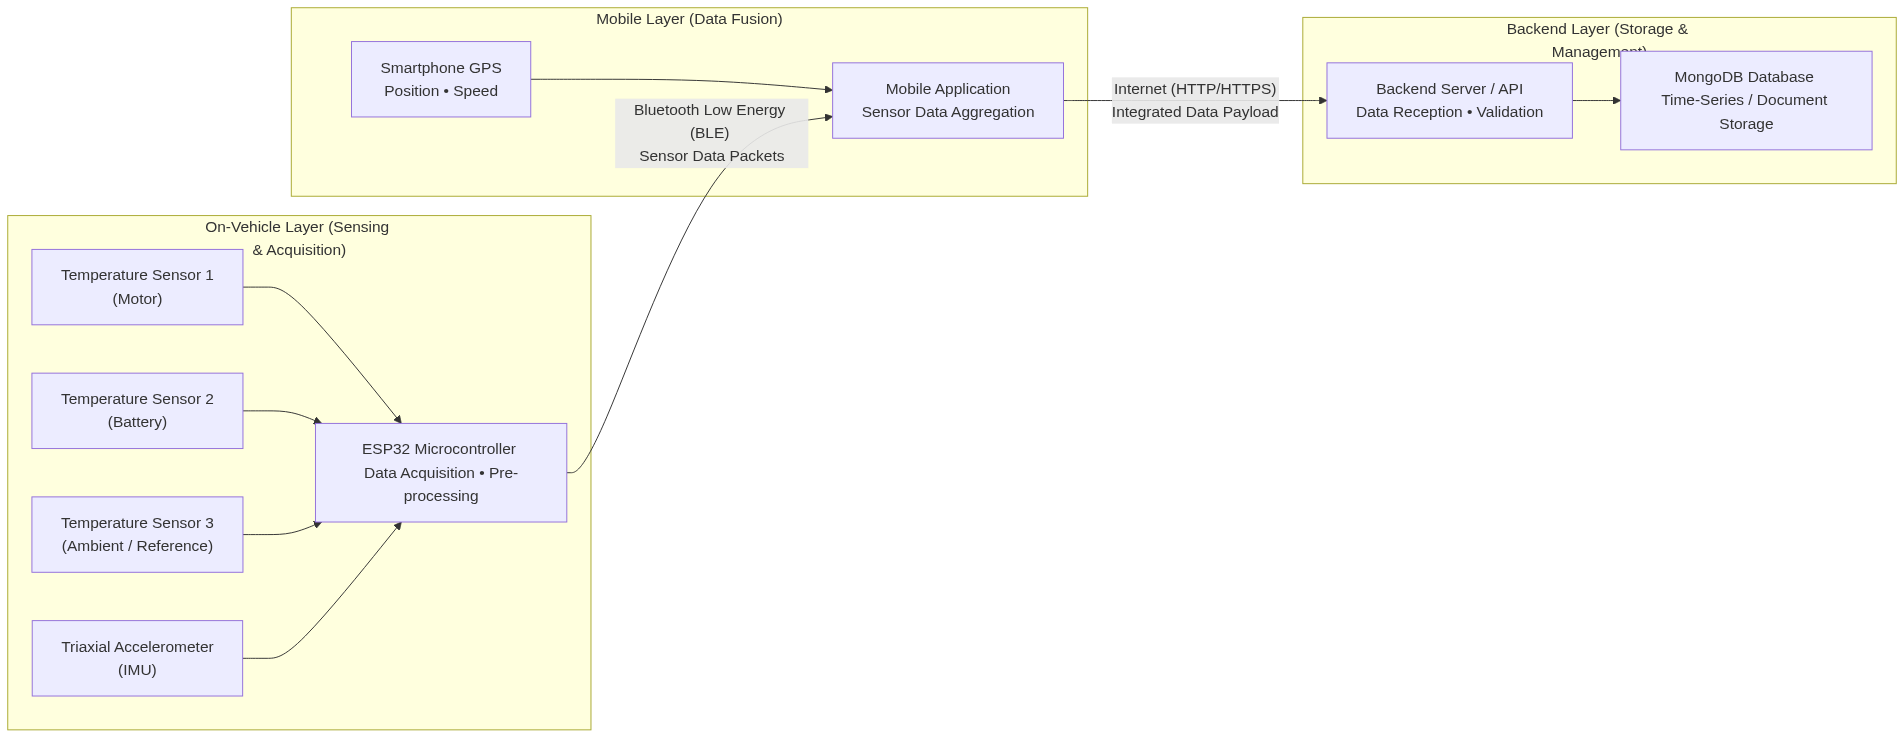
\includegraphics[width=\columnwidth]{img/data-architecture.png}
\caption{Overview of the proposed data acquisition and processing architecture, integrating external sensors, mobile device, and backend infrastructure.}
\label{fig:data-architecture}
\end{figure}

The sensing layer comprised three external digital temperature sensors of type DS18B20, mounted on accessible surfaces to avoid invasive instrumentation. These sensors were used to measure the surface temperature of the battery casing, the surface temperature of the electric motor, and an ambient reference temperature. The DS18B20 sensors were selected due to their digital interface, acceptable accuracy for thermal monitoring applications, and ease of deployment in outdoor environments. This configuration enables comparative thermal analysis between subsystems and environmental conditions while remaining fully independent of the internal battery management system and vehicle control electronics.

\begin{figure}[!ht]
\centering
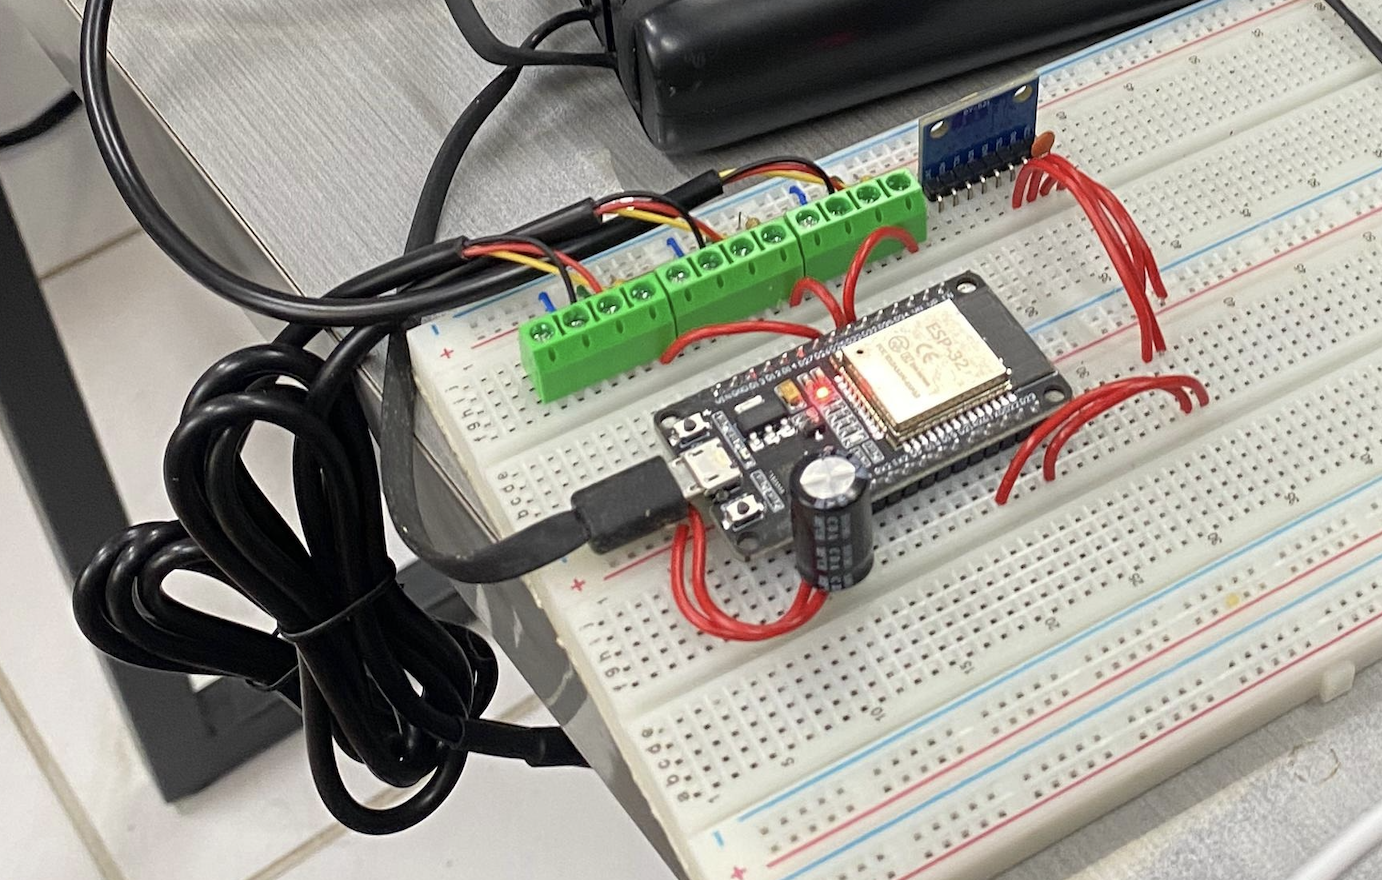
\includegraphics[width=\columnwidth]{img/cicuit-sensors.png}
\caption{External sensing unit (ESP32-based prototype) and attached sensors (DS18B20 + IMU).}
\label{fig:prototype}
\end{figure}

In addition to thermal sensing, a triaxial accelerometer module MPU-6050 was employed to capture acceleration and vibration patterns along three axes. The accelerometer data provide complementary information about the vehicle’s dynamic operating regime, which may influence thermal behavior during different riding conditions.

Communication between the embedded processing unit and the intermediate node was established via the Bluetooth Low Energy protocol, enabling continuous data transmission with low power consumption. A mobile device acted as a data concentrator and gateway, receiving telemetry from the ESP32 and enriching it with geolocation and instantaneous speed information obtained via the device’s GPS during vehicle operation. Subsequently, the consolidated dataset was transmitted to a backend server and persisted in a MongoDB non relational database. This architectural choice was adopted to facilitate efficient management of time series data and to support scalability for subsequent analytical processing.

\subsection{Machine Learning Models for Thermal Forecasting}

Thermal analysis was formulated as a supervised regression and forecasting problem, aiming to predict future battery surface temperature values based on historical external measurements. Multiple machine learning algorithms were evaluated to model the nonlinear relationships between thermal, kinematic, and contextual variables.

The K Nearest Neighbors (KNN) algorithm was employed due to its nonparametric nature and intuitive assumption that similar operating states lead to similar thermal behavior. KNN does not construct an explicit model during training, instead storing the training dataset and computing predictions based on the proximity of new observations to historical samples. This characteristic makes it effective at capturing local thermal patterns under similar driving conditions.

Decision Tree regression was adopted as an interpretable baseline model. The algorithm recursively partitions the feature space into homogeneous regions using decision rules, resulting in a hierarchical structure that maps input conditions to temperature predictions. Its transparency and low computational complexity make it suitable for scenarios where model interpretability and potential embedded deployment are relevant.

Random Forest regression was used to address the limitations of single decision trees, particularly their tendency to overfit. By aggregating the predictions of multiple trees trained on random subsets of data and features, Random Forest provides improved robustness to noise and variability, which are common in real-world sensor data.

Gradient Boosting was also evaluated as an ensemble learning approach. Gradient Boosting constructs trees sequentially, with each new model trained to minimize the residual error of previous iterations using gradient based optimization. Its optimized architecture makes it effective for capturing complex nonlinear relationships in tabular datasets.

Finally, a Multilayer Perceptron (MLP) neural network was considered to model nonlinear dependencies between input variables and battery temperature. The MLP consists of an input layer, one or more hidden layers, and an output layer, with parameters learned through backpropagation. Its ability to approximate complex functions makes it suitable for modeling thermal dynamics influenced by multiple interacting variables.

\subsection{Experimental Data Collection Protocol}

The experimental data collection was conducted using an electric motorcycle instrumented with the sensing system described in the previous section and connected to a smartphone for GPS based data acquisition. The mobile device was used to record geolocation and instantaneous speed throughout the experiments, enabling spatial and contextual characterization of the vehicle’s operation. Three external digital temperature sensors were installed to monitor ambient temperature, electric motor surface temperature, and battery casing surface temperature, allowing simultaneous observation of thermal behavior across different subsystems.

\begin{figure}[!ht]
\centering
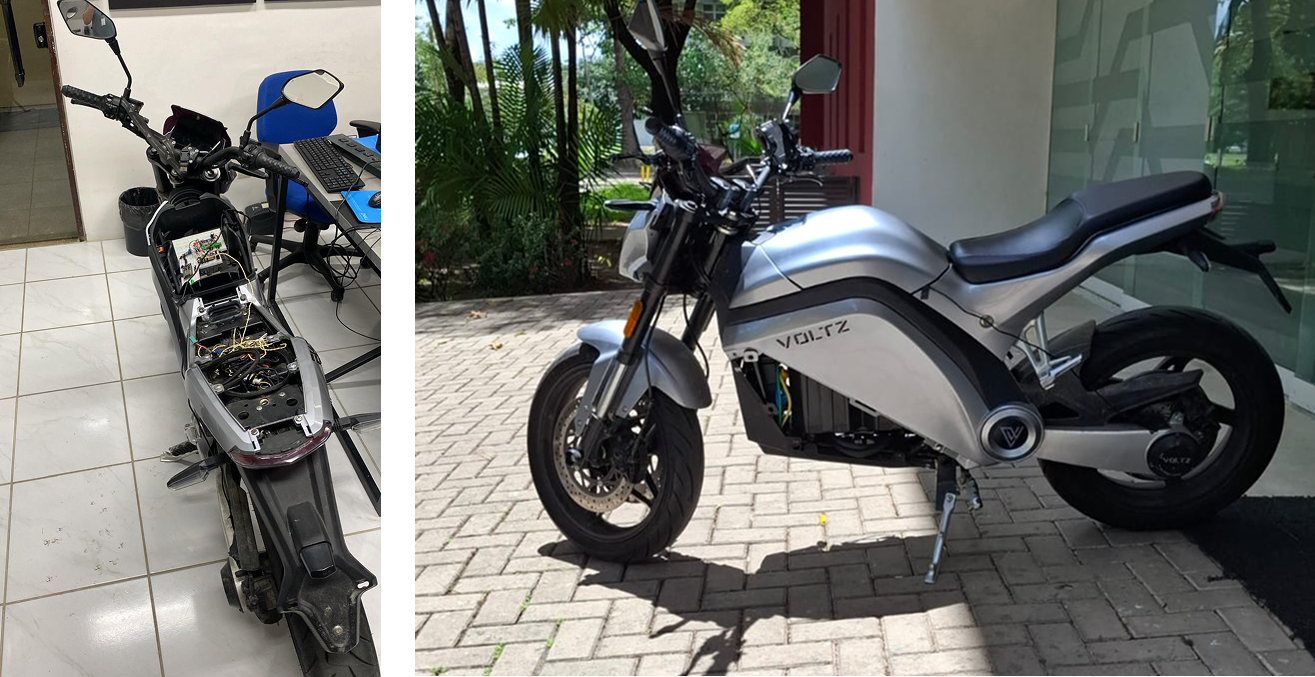
\includegraphics[width=\columnwidth]{img/motocycle.png}
\caption{Experimental platform: electric motorcycle instrumented with external sensing system.}
\label{fig:motorcycle}
\end{figure}

Data were collected during real-world riding sessions carried out on predefined routes, selected to reflect typical urban operating conditions. The experiments were conducted on the UFPE campus in Recife, Brazil, using routes that include variations in speed, acceleration, stops, and road topology. Each experimental run had an approximate duration of ten minutes, ensuring sufficient temporal coverage to capture gradual thermal evolution during vehicle operation.

To induce variability in operational load and thermal behavior, the motorcycle was configured in distinct driving modes across different runs. These modes resulted in different power delivery profiles and riding dynamics, contributing to diverse thermal responses. The use of multiple driving modes and repeated routes allowed the dataset to capture a range of realistic operating scenarios rather than isolated or controlled laboratory conditions.

The predefined routes were consistently followed across experiments to ensure comparability between runs. Geolocation data recorded by the smartphone were later used to reconstruct the trajectories and generate route maps corresponding to each experimental session. These maps provide spatial context for the collected telemetry and support the analysis of thermal behavior in relation to riding conditions and route characteristics. The inclusion of route maps also contributes to experimental transparency and reproducibility by explicitly documenting the circuits used during data collection.

\begin{figure}[!ht]
\centering
\subfloat[Eco]{%
  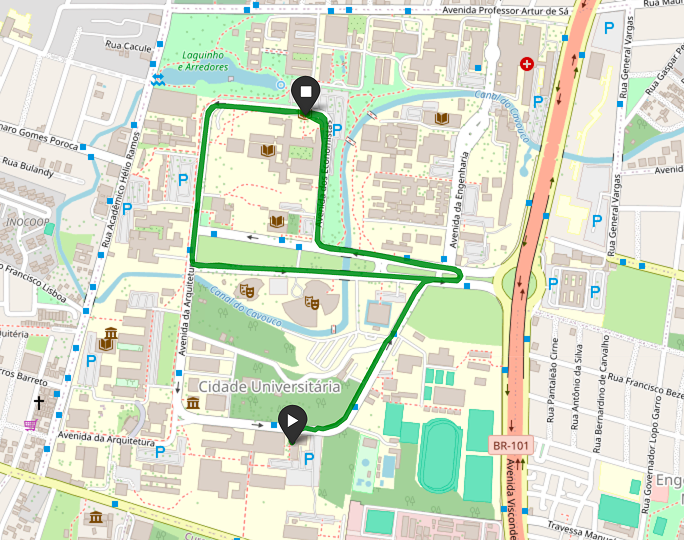
\includegraphics[width=0.90\columnwidth]{img/map-eco.png}%
  \label{fig:map-eco}%
}\\[0.6em]
\subfloat[Normal]{%
  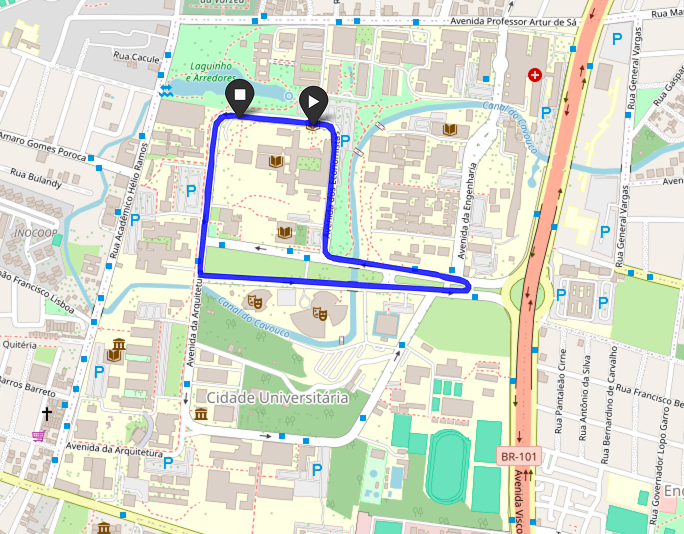
\includegraphics[width=0.90\columnwidth]{img/map-nor.png}%
  \label{fig:map-nor}%
}\\[0.6em]
\subfloat[Turbo]{%
  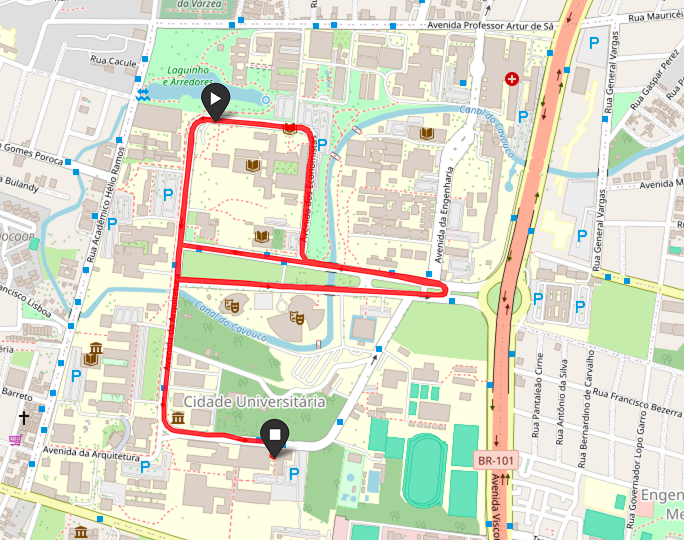
\includegraphics[width=0.90\columnwidth]{img/map-tur.png}%
  \label{fig:map-tur}%
}
\caption{Reconstructed experimental routes for each driving mode (Eco, Normal, Turbo), used to contextualize operational conditions and improve reproducibility.}
\label{fig:routes}
\end{figure}

\subsection{Data Preprocessing}

Raw telemetry data were exported from the database and consolidated into a structured dataset prior to analysis. The dataset included timestamps, geographic coordinates, instantaneous speed, accelerometer measurements, and temperature readings.

In the preprocessing stage, categorical variables related to driving mode were encoded numerically, and elapsed time variables were computed to normalize each experimental run. Data cleaning procedures were applied to remove administrative identifiers and variables without physical relevance to thermal behavior. Temperature readings associated with sensor communication failures or physically implausible values were filtered out.

Variables were renamed for standardization, and the feature vector consisted of ambient temperature, speed, acceleration components, driving mode, and elapsed time. Battery surface temperature was defined as the target variable. The dataset was then split into training and test subsets following an eighty twenty ratio to support evaluation of model generalization.

\subsection{Software Environment and Model Training}

The entire data processing and modeling workflow was implemented in Python using a notebook based environment. Data manipulation and time series handling were performed using pandas and NumPy. Machine learning models were implemented using the Scikit learn framework, while Gradient Boosting was employed for gradient boosting regression.

Feature normalization was performed using StandardScaler to ensure zero mean and unit variance, a necessary condition for distance based and gradient based models. Hyperparameter optimization was conducted using RandomizedSearchCV with cross validation, allowing efficient exploration of the parameter space for each algorithm.

During model training and optimization, a background monitoring routine was executed to record execution time, CPU usage, and memory consumption. This allowed analysis of the trade off between predictive performance and computational cost. The best estimator obtained from the optimization process was retrained on the full training dataset and evaluated on the unseen test set.

\subsection{Forecasting-Based Thermal Risk Assessment}


Rather than performing direct fault classification, thermal risk assessment was derived from temperature forecasting results. Each model was trained to predict near future battery surface temperature values based on historical input sequences.

Potential anomalies or overheating risks were inferred by comparing forecasted temperature trajectories against predefined safety thresholds associated with battery operation. Sustained predicted temperature growth or threshold exceedance was interpreted as an early indicator of abnormal thermal behavior.

This forecasting-based approach enables anticipatory detection of thermal risks without reliance on labeled fault data or internal vehicle signals, aligning with the objective of external, non intrusive monitoring.

\section{Results}

\subsection{Dataset Description}

The final dataset was composed of telemetry collected during real-world riding experiments conducted under three distinct driving modes. After preprocessing and removal of invalid samples, the dataset contained approximately one thousand synchronized records. Each record included battery surface temperature, ambient temperature, vehicle speed, triaxial acceleration measurements, elapsed time since the beginning of the ride, and the operating mode.

\begin{table}[!ht]
\centering
\scriptsize
\caption{Descriptive statistics for the main variables (raw exploratory output).}
\label{tab:desc-stats}
\resizebox{\columnwidth}{!}{%
\begin{tabular}{lrrrrrrrr}
\toprule
Variable & Count & Mean & Std & Min & 25\% & 50\% & 75\% & Max \\
\midrule
temp\_battery & 1006.0 & 33.663082 & 0.886562 & 32.69 & 32.810000 & 33.380000 & 34.380000 & 35.620000 \\
speed         & 1006.0 &  9.031026 & 4.271617 &  0.00 &  5.885671 &  9.318798 & 12.169095 & 19.051404 \\
accX          & 1006.0 & 1096.579523 & 233.007021 & 167.00 & 970.000000 & 1097.000000 & 1206.750000 & 2808.000000 \\
temp\_amb     & 1006.0 & 31.884920 & 0.489337 & 30.44 & 31.560000 & 31.880000 & 32.250000 & 33.120000 \\
\bottomrule
\end{tabular}%
}
\end{table}

The data were sampled continuously throughout the experimental sessions, resulting in time series that capture gradual thermal evolution rather than isolated operating points. Minor data losses were observed, primarily associated with transient communication or sensor reading issues. These occurrences were limited in number and did not compromise the temporal continuity of the dataset after preprocessing.

The resulting dataset reflects realistic operational variability, including periods of acceleration, cruising, stops, and speed fluctuations, providing a representative basis for thermal behavior analysis and forecasting.

\subsection{Battery Thermal Behavior}

Across all experimental runs, the battery surface temperature exhibited a gradual and monotonic increase during vehicle operation. Temperature evolution followed a smooth trajectory, consistent with the thermal inertia expected from battery systems.

\begin{figure}[!ht]
\centering
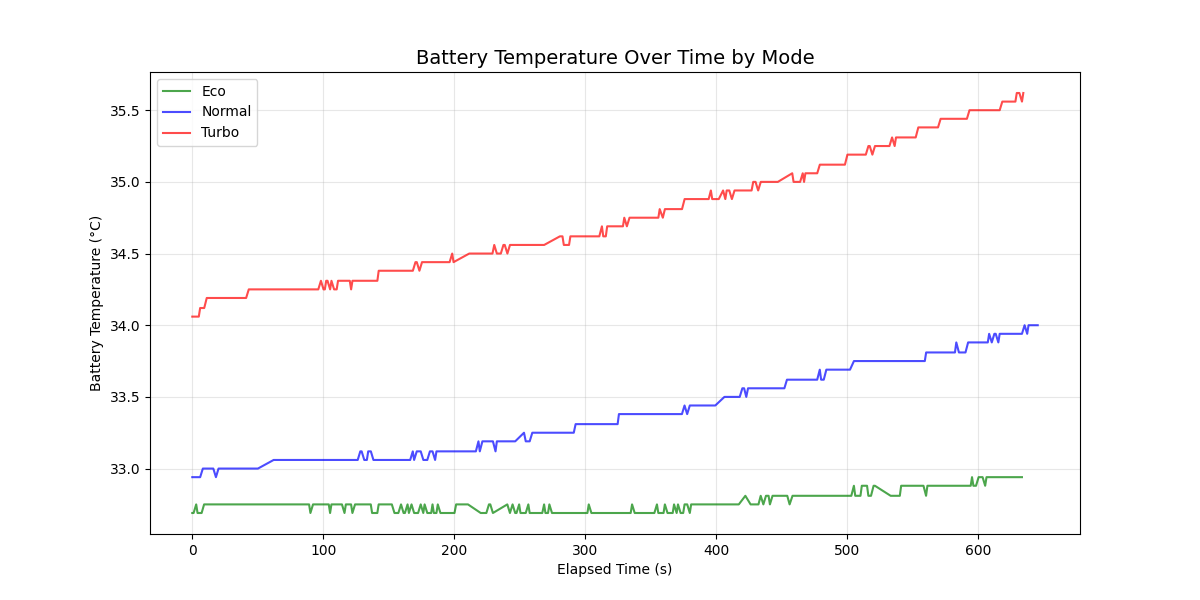
\includegraphics[width=\columnwidth]{img/battery_eda_evolucao_temp_tratados.png}
\caption{Battery surface temperature evolution over time for each driving mode.}
\label{fig:temp-evolution}
\end{figure}

Clear differences in absolute temperature levels were observed between driving modes. Runs conducted under higher power demand modes showed higher battery surface temperatures over time, while lower demand modes exhibited more stable thermal profiles with smaller temperature increments.

\begin{figure}[!ht]
\centering
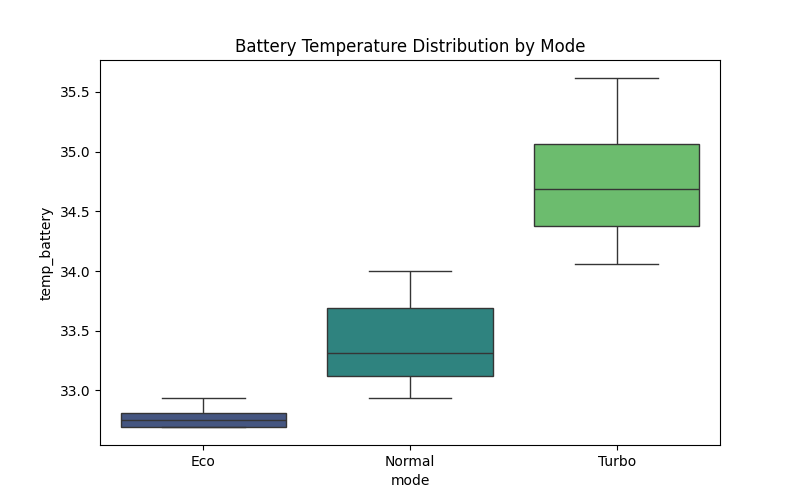
\includegraphics[width=\columnwidth]{img/battery_eda_boxplot_temp_tratados.png}
\caption{Battery temperature distribution across operating modes.}
\label{fig:temp-boxplot}
\end{figure}

The battery temperature remained within a relatively narrow range across all experiments, with no abrupt spikes or discontinuities once sensor outliers were removed. This behavior indicates stable thermal operation during the monitored sessions and provides a consistent baseline for forecasting analysis.

\subsection{Influence of Operating Conditions}

Operating conditions had a visible influence on battery thermal behavior. Driving mode was strongly associated with differences in temperature trajectories, with higher performance modes resulting in higher average battery temperatures and steeper thermal gradients.

Vehicle speed and elapsed time showed a positive association with battery temperature evolution, reflecting cumulative energy usage over the duration of the ride. Ambient temperature exhibited a weaker but observable relationship with battery surface temperature, contributing to baseline thermal levels rather than short-term variations.

Acceleration and vibration signals presented lower direct correlation with instantaneous battery temperature. However, these signals contributed indirectly by characterizing the operational regime and temporal dynamics of the vehicle.

Correlation analysis confirmed that no single variable fully explained battery temperature behavior, reinforcing the multivariate nature of the thermal process.

\begin{figure}[!ht]
\centering
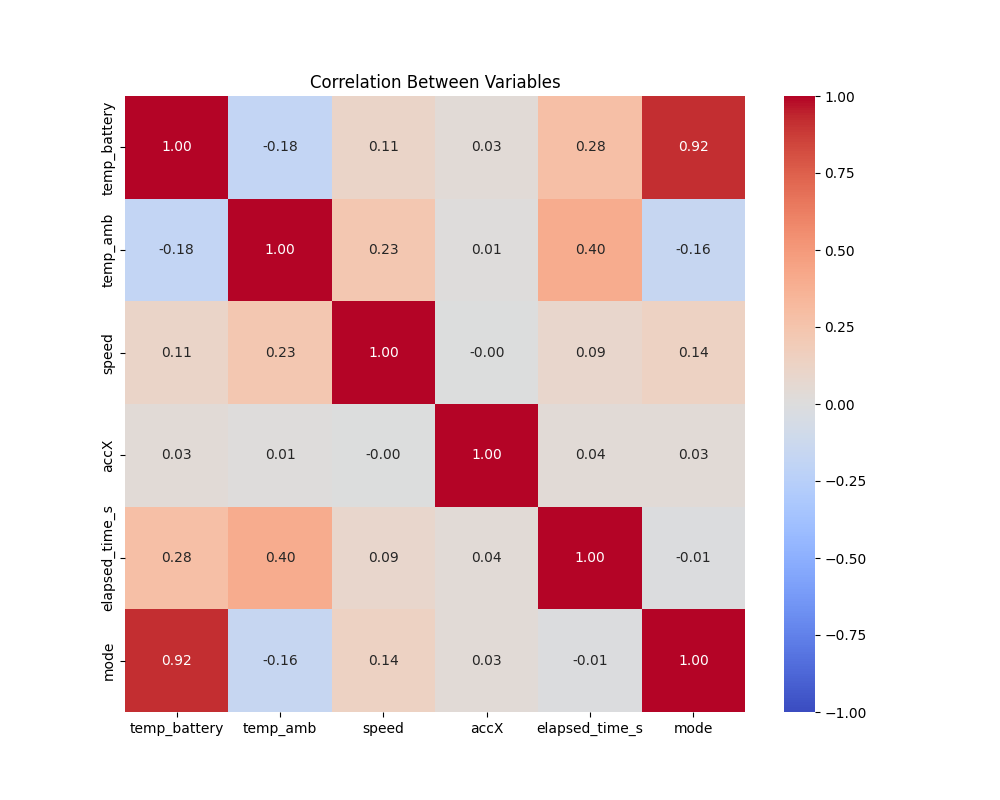
\includegraphics[width=\columnwidth]{img/battery_eda_correlacao_tratados.png}
\caption{Correlation matrix between battery temperature and operational variables.}
\label{fig:corr-matrix}
\end{figure}

\subsection{Observed Thermal Irregularities}

During the initial exploratory analysis of raw sensor data, isolated anomalous temperature readings were identified. These anomalies were characterized by physically implausible values and abrupt deviations from the surrounding measurements.

Such anomalies were attributed to transient sensor communication failures rather than genuine thermal events. After applying data cleaning procedures and filtering outliers, the resulting time series no longer exhibited spurious temperature drops or spikes.

No sustained abnormal thermal behavior or overheating events were observed during the experimental runs. The absence of extreme thermal events provides a stable reference scenario for evaluating early risk detection through forecasting rather than fault classification.

\subsection{Temperature Forecasting Performance}

Multiple machine learning models were evaluated for battery temperature prediction, including distance-based, tree-based, ensemble, and neural network approaches. Forecasting performance varied across models and feature configurations.

Table~II summarizes forecasting performance metrics across models, while Table~III reports the observed computational cost during training.

\begin{table}[!ht]
\centering
\caption{Forecasting performance comparison across evaluated models using the treated dataset.}
\label{tab:model-performance}
\scriptsize
\setlength{\tabcolsep}{4pt}
\begin{tabular}{lcccc}
\toprule
Model & $R^2$ & MAE & RMSE & Train Time (s) \\
\midrule
Random Forest      & 0.9994 & 0.0124 & 0.0214 & 0.990 \\
Decision Tree      & 0.9992 & 0.0124 & 0.0248 & 0.104 \\
Gradient Boosting  & 0.9984 & 0.0236 & 0.0346 & 0.763 \\
MLP                & 0.9899 & 0.0652 & 0.0864 & 2.200 \\
KNN                & 0.9747 & 0.0725 & 0.1370 & 0.110 \\
\bottomrule
\end{tabular}
\end{table}

\begin{table}[!ht]
\centering
\caption{Computational cost during training for each model on the treated dataset.}
\label{tab:compute-cost}
\scriptsize
\setlength{\tabcolsep}{4pt}
\begin{tabular}{lccc}
\toprule
Model & Train Time (s) & CPU (\%) & RAM (MB) \\
\midrule
Random Forest     & 0.990 & 4.92  & 1735 \\
Decision Tree     & 0.104 & 9.86  & 1734 \\
Gradient Boosting & 0.763 & 10.80 & 1624 \\
MLP               & 2.200 & 2.16  & 1511 \\
KNN               & 0.110 & 9.29  & 1809 \\
\bottomrule
\end{tabular}
\end{table}

\begin{figure}[!ht]
\centering
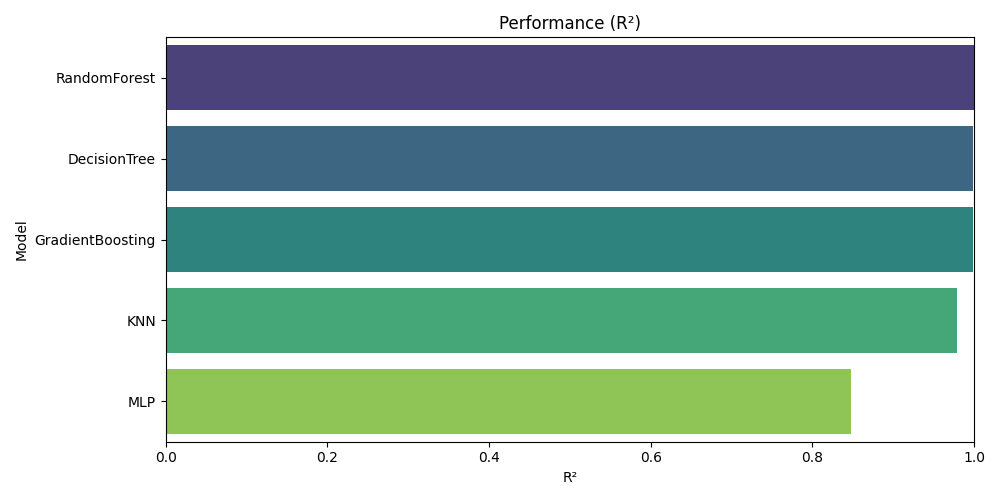
\includegraphics[width=\columnwidth]{img/battery_performance_modelos_tratados.png}
\caption{Comparison of forecasting performance across evaluated machine learning models.}
\label{fig:model-performance}
\end{figure}

When trained on raw instantaneous features, several models exhibited limited predictive capability, reflected in higher prediction errors and reduced goodness-of-fit metrics. The inclusion of temporal features capturing thermal inertia, such as rolling averages and cumulative indicators, led to substantial improvements in forecasting accuracy across most models.

Tree-based ensemble models and neural network models demonstrated consistent alignment between predicted and observed temperature trajectories on unseen test data. Simpler models showed higher sensitivity to noise and local fluctuations.

Overall, the results indicate that battery surface temperature can be forecast with high fidelity when temporal context is incorporated into the feature representation.

\subsection{Early Overheating Detection}

Forecasted temperature trajectories were compared against predefined safety thresholds to assess early overheating detection capability. In all experimental runs, predicted temperatures remained below critical limits, consistent with the absence of observed overheating events.

Although no critical events occurred, the forecasting models successfully captured upward thermal trends ahead of time, demonstrating their ability to anticipate temperature evolution rather than merely react to threshold crossings.

These observations support the feasibility of using forecasting-based approaches to provide early thermal risk awareness using only external, non-intrusive sensor data, even in the absence of labeled fault conditions.

\section{Discussion}

\subsection{Comparison with Existing Literature}

The thermal behavior observed in this study is consistent with prior research that identifies temperature evolution as a central indicator of battery safety and degradation. Numerous works on battery thermal monitoring and anomaly detection rely primarily on internal Battery Management System (BMS) signals, laboratory-instrumented cells, or physics-based electrochemical–thermal models to estimate internal temperature and predict thermal runaway (Xie et al., 2017; Feng et al., 2018; Srinivasan et al., 2019). These approaches typically assume direct access to internal parameters such as core temperature, internal resistance, or heat generation rates, and are often validated under controlled experimental conditions rather than real-world operation.

The gradual and smooth temperature trajectories observed in this study align with the thermal inertia reported in both mechanism-based and data-driven studies (Chen et al., 2020; Li et al., 2023), reinforcing that battery thermal dynamics evolve continuously rather than through abrupt transitions under normal operation. Unlike traditional sensor-threshold methods, which primarily detect faults after abnormal conditions have already manifested (Nascimento et al., 2020), the forecasting-based strategy adopted here focuses on anticipating temperature evolution. This aligns conceptually with recent prognostic frameworks that combine temperature prediction with abnormality detection to provide earlier warning horizons (Hong et al., 2019; Li et al., 2023).

However, most existing forecasting-based methods depend on richer internal sensing, large-scale historical datasets, or vehicle-integrated monitoring infrastructures (Yu et al., 2021; Li et al., 2023). In contrast, the present results demonstrate that meaningful early thermal trend awareness can be achieved using only externally measured surface temperature and operational signals collected under real-world riding conditions. While this does not provide direct equivalence to internal temperature estimation or thermal runaway prognosis, it complements existing BMS-centric approaches by offering a lightweight and deployable alternative for scenarios where internal access is limited or unavailable.

\subsection{Justification for External Non-Intrusive Sensors}

The findings provide empirical support for the feasibility of relying exclusively on external, non-intrusive temperature sensing. Prior studies have highlighted the high cost and integration complexity associated with invasive sensing solutions, such as embedded fiber-optic temperature networks or additional internal probes (Yu et al., 2021). Moreover, dependence on proprietary BMS data restricts applicability across different manufacturers and vehicle generations.

Despite these limitations, the consistency of the observed thermal patterns across operating modes and the forecasting models’ ability to track and anticipate temperature trends indicate that external surface measurements can capture relevant thermal information. Similar conclusions have been suggested in studies that analyze surface or probe temperatures as indirect indicators of internal thermal behavior (Chen et al., 2019; Hong et al., 2019), particularly when combined with contextual operational data.

From a deployment perspective, external sensing offers clear advantages: ease of installation, independence from proprietary vehicle systems, and suitability for retrofitting existing fleets. The results of this study reinforce the notion that external monitoring can function as a complementary or redundant safety layer, enhancing thermal awareness without modifying internal vehicle architectures.

\subsection{Advantages and Limitations of the Proposed Approach}

Several strengths of the proposed approach are evident when compared to existing literature. First, the forecasting models demonstrated robustness to minor data losses and measurement noise, a known challenge in real-world vehicular telemetry (Li et al., 2023). The incorporation of temporal features enabled the models to capture gradual thermal trends, which are often overlooked by instantaneous threshold-based methods (Nascimento et al., 2020).

Additionally, the absence of reliance on labeled fault data represents an advantage in safety-critical domains where abnormal events are rare and difficult to collect ethically or experimentally. This contrasts with supervised fault-classification approaches that require extensive fault datasets obtained under laboratory-induced failure scenarios (Feng et al., 2018; Cai et al., 2020).

Nevertheless, important limitations must be acknowledged. External surface temperature is an indirect proxy for internal battery temperature and may lag or attenuate internal thermal events, particularly during rapid fault escalation. Sensor placement has a critical influence, as variations in airflow, mechanical shielding, or local heating can affect measurements, an issue also noted in prior surface-based monitoring studies (Chen et al., 2019). Environmental conditions further introduce variability, potentially confounding thermal interpretation if not adequately represented in the data.

Moreover, the experimental dataset was limited in size and vehicle diversity, reflecting a single platform and a restricted range of operating conditions. While sufficient to demonstrate feasibility, this limits generalization when compared to large-scale studies based on fleet-level or multi-year datasets (Li et al., 2023). The absence of observed overheating or thermal runaway events also restricts conclusions to early trend awareness rather than validated fault or failure prognosis.

\subsection{Practical Applicability and Real-World Implications}

Despite these constraints, the results highlight several practical implications. The proposed approach is well suited to fleet monitoring scenarios, where low-cost external sensors and lightweight forecasting models can provide continuous thermal oversight without integration into proprietary vehicle electronics. Similar motivations have been discussed in recent works emphasizing scalable, data-driven safety monitoring for real-world electric vehicles (Hong et al., 2019; Li et al., 2023).

For existing electric vehicle fleets, particularly in shared mobility or delivery contexts, the non-intrusive nature of the system facilitates retrofitting and cross-platform deployment. Even without direct internal temperature estimation, early awareness of abnormal thermal trends can support preventive maintenance and conservative operational strategies, potentially reducing safety risks without requiring invasive system access.

However, practical deployment would require addressing challenges related to sensor calibration, long-term drift, data transmission reliability, and model adaptation across different vehicles and environments. Integration with fleet management platforms and alignment with operational safety protocols are also necessary to translate predictive insight into actionable decisions.

Overall, the findings suggest that external, forecasting-based thermal monitoring constitutes a viable and pragmatic complement to existing BMS-based approaches. Rather than positioning the method as a universal replacement, it should be viewed as an additional safety layer that enhances thermal situational awareness under realistic sensing and deployment constraints.

\begin{thebibliography}{00}
\bibitem{b1} H. Togun, A. Basen, J. M. Dhabab, \textit{et al.}, ``A comprehensive review of battery thermal management systems for electric vehicles: Enhancing performance, sustainability, and future trends,'' \textit{International Journal of Hydrogen Energy}, vol. 97, no. 5, pp. 1077--1107, Jan. 2025, doi: 10.1016/j.ijhydene.2024.11.093.
\bibitem{b2} D. Tan \textit{et al.}, ``Study on the thermal characteristics of in-wheel motor drive system based on driving cycles,'' \textit{IEEE Access}, vol. 7, pp. 14463--14471, Dec. 2018, doi: 10.1109/ACCESS.2018.2887143.
\bibitem{b3} A. Boglietti \textit{et al.}, ``Evolution and modern approaches for thermal analysis of electrical machines,'' \textit{IEEE Transactions on Industrial Electronics}, vol. 56, no. 3, pp. 871--882, Mar. 2009, doi: 10.1109/TIE.2008.2011622.
\bibitem{b4} W. Kirchga\ss{}ner, O. Wallscheid, and J. Bocker, ``Estimating electric motor temperatures with deep residual machine learning,'' \textit{IEEE Transactions on Power Electronics}, vol. 36, no. 7, pp. 7480--7488, Jul. 2021, doi: 10.1109/TPEL.2020.3045596.
\bibitem{b5} O. Wallscheid, ``Thermal monitoring of electric motors: State-of-the-art review and future challenges,'' \textit{IEEE Open Journal of Industry Applications}, vol. 2, pp. 204--223, 2021, doi: 10.1109/OJIA.2021.3091870.
\bibitem{b6} ``Weather prediction system using KNN classification algorithm,'' \textit{European Journal of Information Technologies and Computer Science}, vol. 2, no. 1, pp. 10--13, 2022, doi: 10.24018/compute.2022.2.1.44.
\bibitem{b7} IBM, ``What is the k-nearest neighbors (KNN) algorithm?'' [Online]. Available: https://www.ibm.com/think/topics/knn
\bibitem{b8} IBM, ``What is a decision tree?'' [Online]. Available: https://www.ibm.com/think/topics/decision-trees
\bibitem{b9} B. Talekar, ``A detailed review on decision tree and random forest,'' \textit{Bioscience Biotechnology Research Communications}, vol. 13, pp. 245--248, 2020, doi: 10.21786/bbrc/13.14/57.
\bibitem{b10} M. Cioch, M. Kulisz, and A. Gola, ``Comparison of machine learning methods in predictive maintenance of machines,'' \textit{Advances in Science and Technology Research Journal}, vol. 19, no. 11, pp. 33--44, Nov. 2025, doi: 10.12913/22998624/208284.
\bibitem{b11} IBM, ``What is random forest?'' [Online]. Available: https://www.ibm.com/think/topics/random-forest
\bibitem{b12} Y. Yang and H. Wang, ``Random Forest-based machine failure prediction: A performance comparison,'' \textit{Applied Sciences}, vol. 15, p. 8841, 2025, doi: 10.3390/app15168841.
\bibitem{b13} M. Wu \textit{et al.}, ``An intelligent predictive maintenance system based on random forest for addressing industrial conveyor belt challenges,'' \textit{Frontiers in Mechanical Engineering}, vol. 10, Dec. 2024, doi: 10.3389/fmech.2024.1383202.
\bibitem{b14} E. Kavlakoglu and E. Russi, ``XGBoost.'' [Online]. Available: https://www.ibm.com/think/topics/xgboost
\bibitem{b15} R. Shwartz-Ziv and A. Armon, ``Tabular data: Deep learning is not all you need,'' \textit{arXiv} preprint, 2021, doi: 10.48550/arXiv.2106.03253.
\bibitem{b16} T. Kotsiopoulos \textit{et al.}, ``Machine learning and deep learning in smart manufacturing: The smart grid paradigm,'' \textit{Computer Science Review}, vol. 40, p. 100341, May 2021, doi: 10.1016/j.cosrev.2020.100341.
\bibitem{b17} F. Aksan, V. Suresh, and P. Janik, ``PV generation prediction using multilayer perceptron and data clustering for energy management support,'' \textit{Energies}, vol. 18, no. 6, p. 1378, Mar. 2025, doi: 10.3390/en18061378.
\bibitem{b18} V. R. Joseph, ``Optimal ratio for data splitting,'' \textit{Statistical Analysis and Data Mining: The ASA Data Science Journal}, vol. 15, no. 4, pp. 531--538, Apr. 2022, doi: 10.1002/sam.11583.
\bibitem{b19} W. McKinney, ``Pandas: A foundational Python library for data analysis and statistics,'' in \textit{Python High Performance Science Computing}, vol. 14, pp. 1--9, 2011.
\bibitem{b20} M. M. Ahsan \textit{et al.}, ``Effect of data scaling methods on machine learning algorithms and model performance,'' \textit{Technologies}, vol. 9, no. 3, p. 52, Jul. 2021.
\bibitem{b21} L. Yang and A. Shami, ``On hyperparameter optimization of machine learning algorithms: Theory and practice,'' \textit{Neurocomputing}, vol. 415, pp. 295--316, Nov. 2020.
\bibitem{b22} A. Vabalas \textit{et al.}, ``Machine learning algorithm validation with a limited sample size,'' \textit{PLOS ONE}, vol. 14, no. 11, p. e0224365, Nov. 2019.
\bibitem{b23} S. Kishore \textit{et al.}, ``Temperature prediction for electric vehicles using machine learning algorithms,'' \textit{IEEE Transactions on Industry Applications}, vol. 60, no. 6, pp. 9251--9259, Sep. 2024.
\bibitem{b24} D. Bora, D. Singh, and B. Negi, ``Utilization of DS18B20 temperature sensor for predictive maintenance of reciprocating compressor,'' in \textit{Proc. 2023 International Conference on Power Energy, Environment \& Intelligent Control (PEEIC)}, Dec. 2023, pp. 147--150.
\bibitem{b25} A. Kowalskie, ``The impact of outliers on linear regression models: Detection and correction strategies,'' \textit{OTS Canadian Journal}, vol. 4, no. 6, pp. 108--118, Jun. 2025.
\bibitem{b26} L. Grinsztajn, E. Oyallon, and G. Varoquaux, ``Why do tree-based models still outperform deep learning on tabular data?'' \textit{arXiv} preprint arXiv:2207.08815, 2022.
\end{thebibliography}

\end{document}
